\documentclass[conference]{IEEEtran}
\usepackage{cite}
\usepackage{amsmath,amssymb,amsfonts}
\usepackage{algorithmic}
\usepackage{graphicx}
\usepackage{hyperref}
\usepackage{textcomp}
\usepackage{xcolor}
\def\BibTeX{{\rm B\kern-.05em{\sc i\kern-.025em b}\kern-.08em
    T\kern-.1667em\lower.7ex\hbox{E}\kern-.125emX}}
\begin{document}

\title{Wildfire Exploratory Visualization and Machine Learning\\}

\author{\IEEEauthorblockN{1\textsuperscript{st} Sidharth Bambah}
\IEEEauthorblockA{\textit{UNI: sb4283}\\
\textit{Electrical Engineering} \\
\textit{Columbia University}\\
New York, USA \\
sidharth.bambah@columbia.edu}
\and
\IEEEauthorblockN{2\textsuperscript{nd} 
Vedant Dave}
\IEEEauthorblockA{\textit{UNI: vad2134}\\
\textit{Electrical Engineering} \\
\textit{Columbia University}\\
New York, USA \\
vad2134@columbia.edu}
}

\maketitle

\begin{abstract}
    Wildfires are a large issue in the United States and cause devastation year after year. This project aims to use a government-funded dataset of wildfire data to generate visualizations for better understanding of wildfire scope, frequency, and causation. Additionally, these visualizations guide the creation of machine learning models using the Random Forest Classifier algorithm to predict the causes of wildfires throughout the United States given user input. \par
    This paper demonstrates the data type conversion and cleaning performed on the wildfire dataset as well as the exploratory analysis and machine learning experiments performed before the creation of models with strong accuracy evaluations for the available data. \par
    The output is presented in the form of a dynamic web application deployed with cloud services. The application supports user input to dynamically generate visualizations for parameters of interest; also, users can provide details of fires and perform causation predictions with the trained models.
    \linebreak
\end{abstract}

\begin{IEEEkeywords}
big data, machine learning, data visualization, flask
\end{IEEEkeywords}

\section{Introduction}
Wildfires are a colossal problem in the United States (US). Every year, these fires cause rampant devastation and leave much destruction in their wake ranging from property damages and injuries to loss of life. It would be immensely useful to understand the causes, amounts, and severity of wildfires within the United States to help make recommendations for government aid spending and even to develop initiatives for preventative measures. \par

The dataset "1.88 Million Wildfires" can help with just that. It contains accurate data of wildfires in the US along with numerous features, which can be exploited for enhanced understanding. \par

While volume, velocity, and variety typically encompass big data, it is important to consider another equally important feature, value \cite{DBLP:journals/corr/abs-1709-07493}. This value can be extracted through poignant visualizations, which can now be easily created with any of the plethora of graphics libraries. After parsing and cleaning the data using prominent big data analytics tools, visualizations can be generated to allow for straightforward analysis of the data. \par

These visualizations can present a means for more predictive analysis. Common machine learning methods can be used with a subset of the data to train comprehensive models. After being refined to a suitable accuracy, these models will allow for accurate prediction of wildfire causation. \par

The aim of this project is to combine both the visualization and the machine learning models in the form of a dynamic web application. This allows for all aspects of the database to be easily represented in one distinct location. Additionally, user's will be able to input parameters of interest and generate visualizations and model predictions specific to their own use case. \par

\section{Related Work}
There are many works which touch upon the topics discussed in this paper. The subjects can be split into a few distinct components, such as wildfire analysis, exploratory visualization, machine learning, and web app deployment. Each of these fields are quite broad; however, the following paragraphs touch on a few publications tightly related to this topic. \par

With regards to wildfire analysis, there is an approach to use probabilistic exposure analysis to identify the likelihood of populate locations coming into contact with a wildfire. Further, a risk matrix is generated to allow planners a method to identify where the risk is spatially and to qualify the major driving factors \cite{HAAS201344}. This work is quite similar in that correlation matrix are used to identify strongly linked features of wildfire properties to develop machine learning models. While not focusing on the risk aspect, simulations can be generated through the visualization to find scale of wildfires across the US. \par

In the field of exploratory visualization, work has been done to introduce 'geowigs', which are a series of geographically weighted interacted graphics that are used to explore spatial relationships \cite{4376135}. This work utilizes a choropleth map in a similar fashion to visualize the scale and amount of wildfires over time in the various states. Further work has been done to discuss the major challenges involved in large scale data analytics as datasets grow two tera- and petabyte sizes \cite{Fisher:2016:BDE:2939502.2939518}. Particularly, the work discusses the issues of computation, rendering, and computation while identifying strategies to handle large scale data \cite{Fisher:2016:BDE:2939502.2939518}. These fundamental design trade-offs are essential to this wildfire work as the dataset contains over 1 million rows and visualizations need to be quickly and efficiently rendered in a web browser. The wildfire project actually utilizes the "look at less of it" presented by this work by allowing for subsets of the data to be utilized during visualization generation. \par

Similarly, in the domain of machine learning, work has been done to compare the performance between support vector machines (SVMs) and random forest classifiers. It concludes that the number of user-defined parameters required by random forest classifiers is less than that needed by SVMs and the parameters in random forest classifiers are easier to define \cite{random_forest_related}. Furthermore, it finds that both machine learning methods perform equally well in terms of classification accuracy and training time \cite{random_forest_related}. These results further help this paper's choice to use a random forest classifier to develop a causation prediction model for wildfires as it allows for accurate predictions, low training time, and fewer required user inputs. \par

Lastly, work in web deployment of big data projects has been done with the processing of radar images. A paper presents an integrated approach to developing full stack software with components such as ReactJS and Apache Spark to allow for quick visualization and algorithmic manipulation of the large radar data \cite{potapovinformation}. This approach is quite similar to that taken by this wildfire work, which also heavily depends on ReactJS for dynamic front-end rendering and a RESTful API to manipulate the dataset. \par

\section{Data}
The dataset used in this work was found on Kaggle and is titled "1.88 Million US Wildfires". The data was compiled by Rachael Tatman and released on Kaggle on September 13, 2017. It also holds a CC0 Public Domain license allowing for open source analysis. \par

The wildfire data includes geo-referenced information of wildfires throughout the entire United States over 24 years, namely from 1992 to 2015. The data was compiled from US federal, state, and local reporting systems. Evidently, it was commissioned by the US government and was originally generated to support the national Fire Program Analysis (FPA) system. \par

For the records to be included in the dataset, they were required to include discovery date, final fire size, and a point location at least as precise as the Public Land Survey System (PLSS) section, which is a 1-square mile grid. Further, whenever possible, the records would have to conform to the standards of the National Wildfire Coordinating Group (NWCG). \par

The data is given as an SQLite database with a size of 759 MB. As mentioned, it has roughly 1.88 million rows, with each row corresponding to a wildfire. The dataset also contains more than thirty features. While not all features are used in this implementation, they allow for a large amount of flexibility in numerous possible extensions. \par

\section{Methods}
\subsection{Data Cleaning}
As mentioned, the dataset is presented in the form of a SQLite database. This is not an easy format to work with, so it was important to put the data into a more useful format and clean any missing values and inconsistencies. All of this data manipulation was performed in a Google Colab notebook with a Python 3 kernel and GPU hardware acceleration. \par

First, the data was read from the database into a Pandas dataframe object. Then, the length of the main table was checked and resulted in 1880465. Clearly, there were around 1.88 million wildfires in the dataset. \par

It turned out that the date feature for each row was given in Julian date format. So, using a pandas date method, a new column was created in the Gregorian date format. This is immensely useful for visualization and easy grouping of the data. Additionally, month and day of week columns were added to provide a few more features for easier data exploration. A sampling of the new cleaned columns, can be seen in Figure \ref{fig:cleaned_data}. \par

\begin{figure}
    \centering
    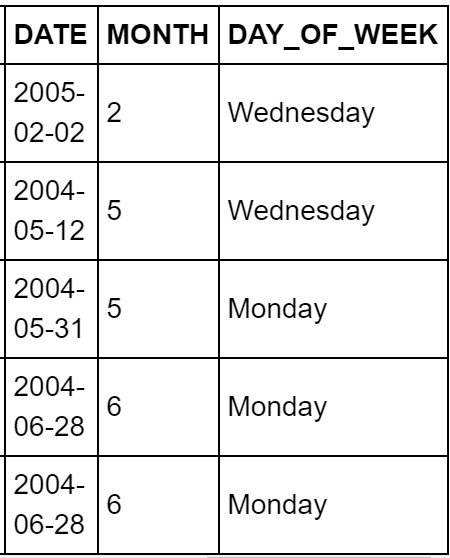
\includegraphics[scale=0.6]{img/cleaned_data.PNG}
    \caption{Sampling of the first five rows of the cleaned and manipulated data using the dataframe .head() method. The Gregorian date, month, and day of week columns have been added for straightforward visualizations.}
    \label{fig:cleaned_data}
\end{figure}

\subsection{Data Exploration}
Before developing a predictive model, it is important to analyze the dataset, find correlations between features, and determine which type of model would be best suited to the data. \par

After the data was cleaned, it was stored into a Pandas dataframe in a Google Colab notebook with a Python 3 kernel and GPU hardware acceleration. Then, simple visualizations were created using the Matplotlib python plotting library. \par

As a straightforward verification of the data, the latitude and longitude points for all of the fire entries were plotted on a scatter plot. Based on the structure of the plot given in Figure \ref{fig:fire_scatter}, it is clear, even without the data overlaid on a US map, that the locations are accurate and represent fires in the US itself.

\begin{figure}
    \centering
    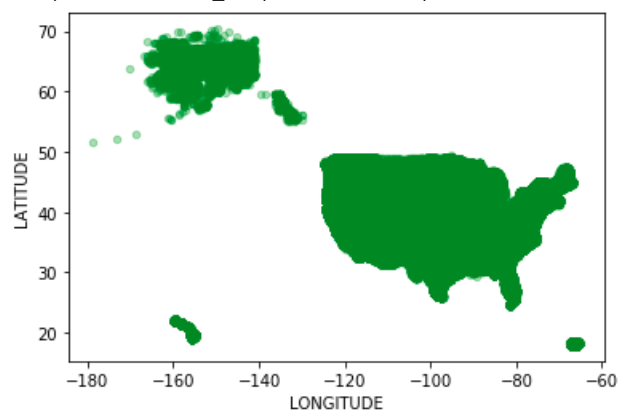
\includegraphics{img/fire_scatter.PNG}
    \caption{Scatter plot of the Latitude and Longitude points for all of the fire entries. Data points resemble the map of the United States even without a geographic underlay.}
    \label{fig:fire_scatter}
\end{figure}

After verifying the data, it was useful to see the distribution of the causes of fires. This is given in Figure \ref{fig:fire_causes} and clearly shows that "debris burning" is the leading cause of fires in the United States over this 24 year period.

\begin{figure}
    \centering
    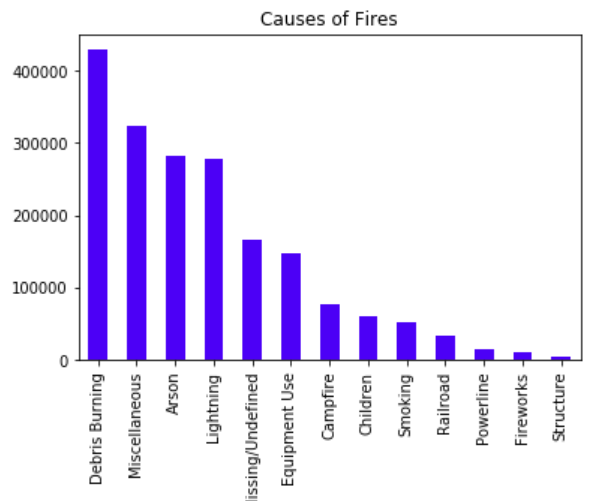
\includegraphics{img/fire_causes.PNG}
    \caption{Distribution of the amount of fires against their causes. "Debris burning" and "Miscellaneous" form the major causes of fires.}
    \label{fig:fire_causes}
\end{figure}

Next, the total numbers of fires was shown for the top ten states. From this, it is evident that, as expected, California, Texas, and Arizona have the largest numbers of fires. This distribution can be seen in Figure \ref{fig:fire_states}. \par

\begin{figure}
    \centering
    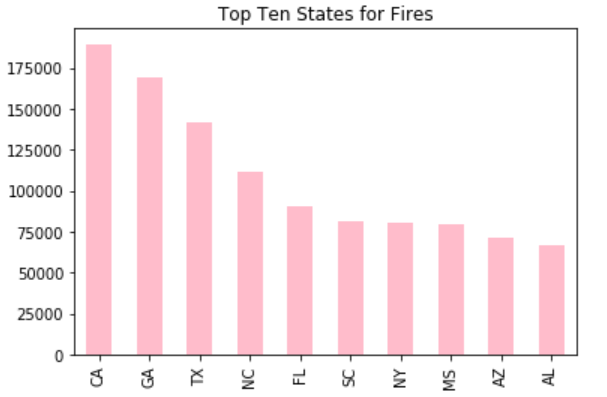
\includegraphics{img/fire_states.PNG}
    \caption{The numbers of fires in each of the top ten states. As expected, California and Texas have the most fires.}
    \label{fig:fire_states}
\end{figure}

Additionally, a correlation matrix was generated to find the ties between the various features of the data. This matrix is given in Figure \ref{fig:correlation_matrix}. The given color bar depicts the relationship between correlation and the color of the cell. The correlation matrix does not include all of the features of the data. Only human understandable and useful classification parameters were kept and things such as element\_id and shape were dropped. Furthermore, the Pearson method was used to generate this matrix, so the categorical variables are excluded as well. \par

\begin{figure}
    \centering
    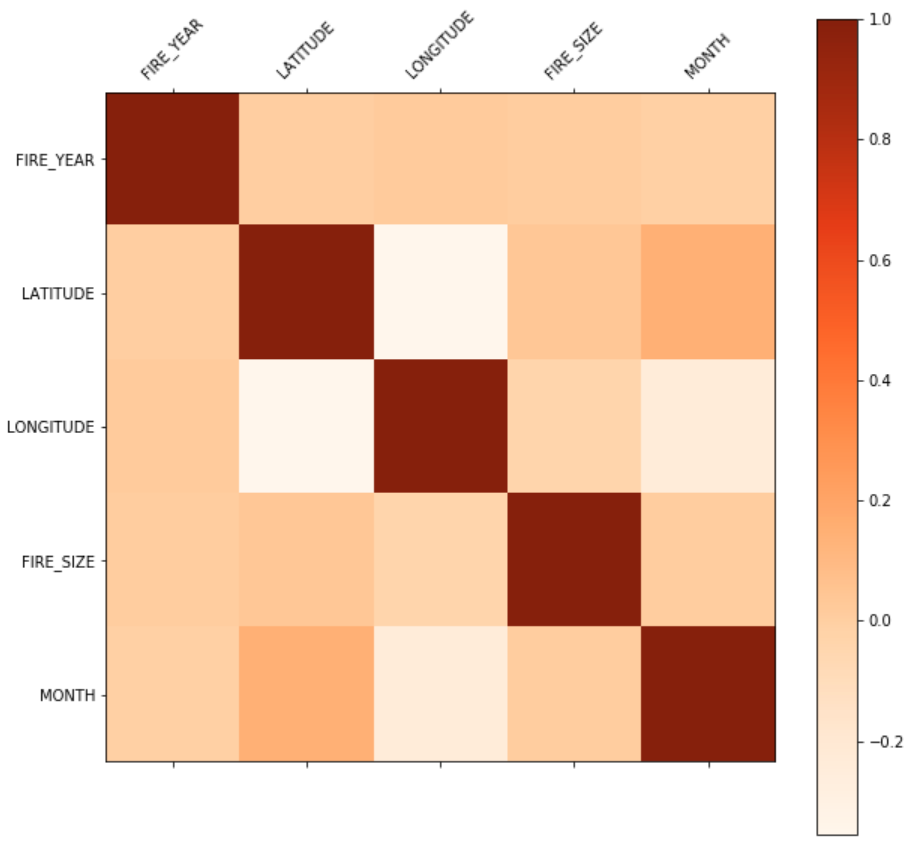
\includegraphics[scale=0.7]{img/correlation_matrix.PNG}
    \caption{Correlation matrix for the features of the data. Only human readable and useful classification features were kept for the matrix generation. There seems to be a correlation between month and latitude as well as fire size and latitude.}
    \label{fig:correlation_matrix}
\end{figure}

\subsection{Machine Learning Model}
After determining the correlations between parameters from data exploration, various methods for machine learning were pursued. The intention is to create a model that can accurately predict the causes of wildfires given user input. \par

The data contains numerous potential causes for the fires. This makes it difficult for accurate predictions due to the many possible outcomes. For simplicity, these categories were condensed into four possible causes: Natural, Accidental, Malicious, and Other. The Natural category includes lightning. The accidental category includes structure, fireworks, power line, railroad, smoking, children, campfire, equipment use, and debris burning. The malicious category includes arson and the final category, other, includes missing/undefined and miscellaneous. \par

After determining this structure, the data was split into a test and training set. Then, a random forest classifier was trained for each of the three states. The features are Latitude, Longitude, Month, and Day of Week. After achieving an accuracy close to 65\%, the prediction authenticity was checked through a classification report that provided the precision, recall, f1-score, and support for all four labels. \par

If a user provides the aforementioned four inputs, the model returns the probabilities of the hypothetical fire being caused by each of the four possible categories. Since a user may not know the latitude and longitude of a location of interest, the application allows free-form location input, which is parsed using the Google Maps Places and Geo-coding APIs. A sample output of the visualization representing predictions is given in Figure \ref{fig:model_predictions}. \par 

\begin{figure}
    \centering
    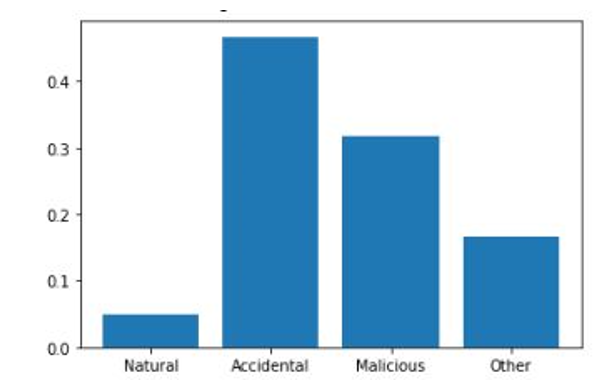
\includegraphics{img/sample_output.PNG}
    \caption{Histogram showing a sample output of the distribution for possible wildfire causes given user input. The data was returned from the trained model.}
    \label{fig:model_predictions}
\end{figure}

\section{Experiments}
\subsection{Visualizations}
The visualizations in the web application were largely created using libraries such as D3, ChartJS, and CanvasJS. They have been deployed in the form of a web application and, as such, are available in a browser. These libraries also allow for high levels of interactivity with the visualizations including hover over, rotation, and on-click effects. \par

The first interesting visualization is a word cloud of the states as a function of the quantity of fires. Essentially, the states with the most fires appear as larger elements of the word cloud and vice versa. This was built as a ReactJS component using the D3 library and can be seen in Figure \ref{fig:wordcloud}.

\begin{figure}
    \centering
    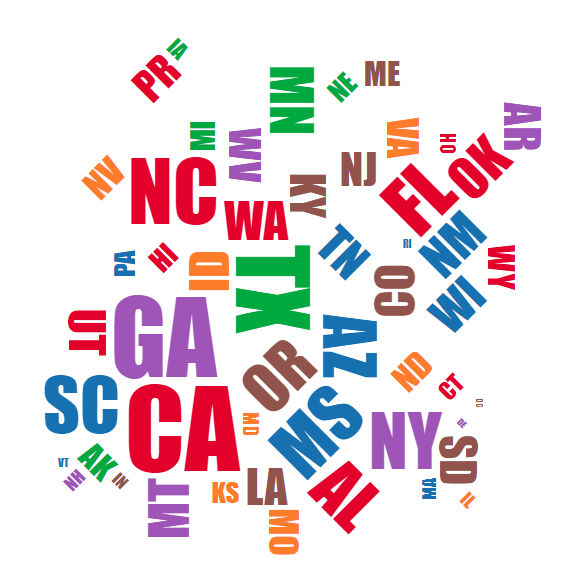
\includegraphics{img/wordcloud.PNG}
    \caption{Word cloud of the states as a function of fire quantity.}
    \label{fig:wordcloud}
\end{figure}

The next visualization is a choropleth map. This is also made with the D3 library. It shows each state as a shade of red. The deeper red colors are for states which have the most fires and vice versa. The states with an unknown number of fires are given in black. This map can be seen in Figure \ref{fig:choropleth}.

\begin{figure}
    \centering
    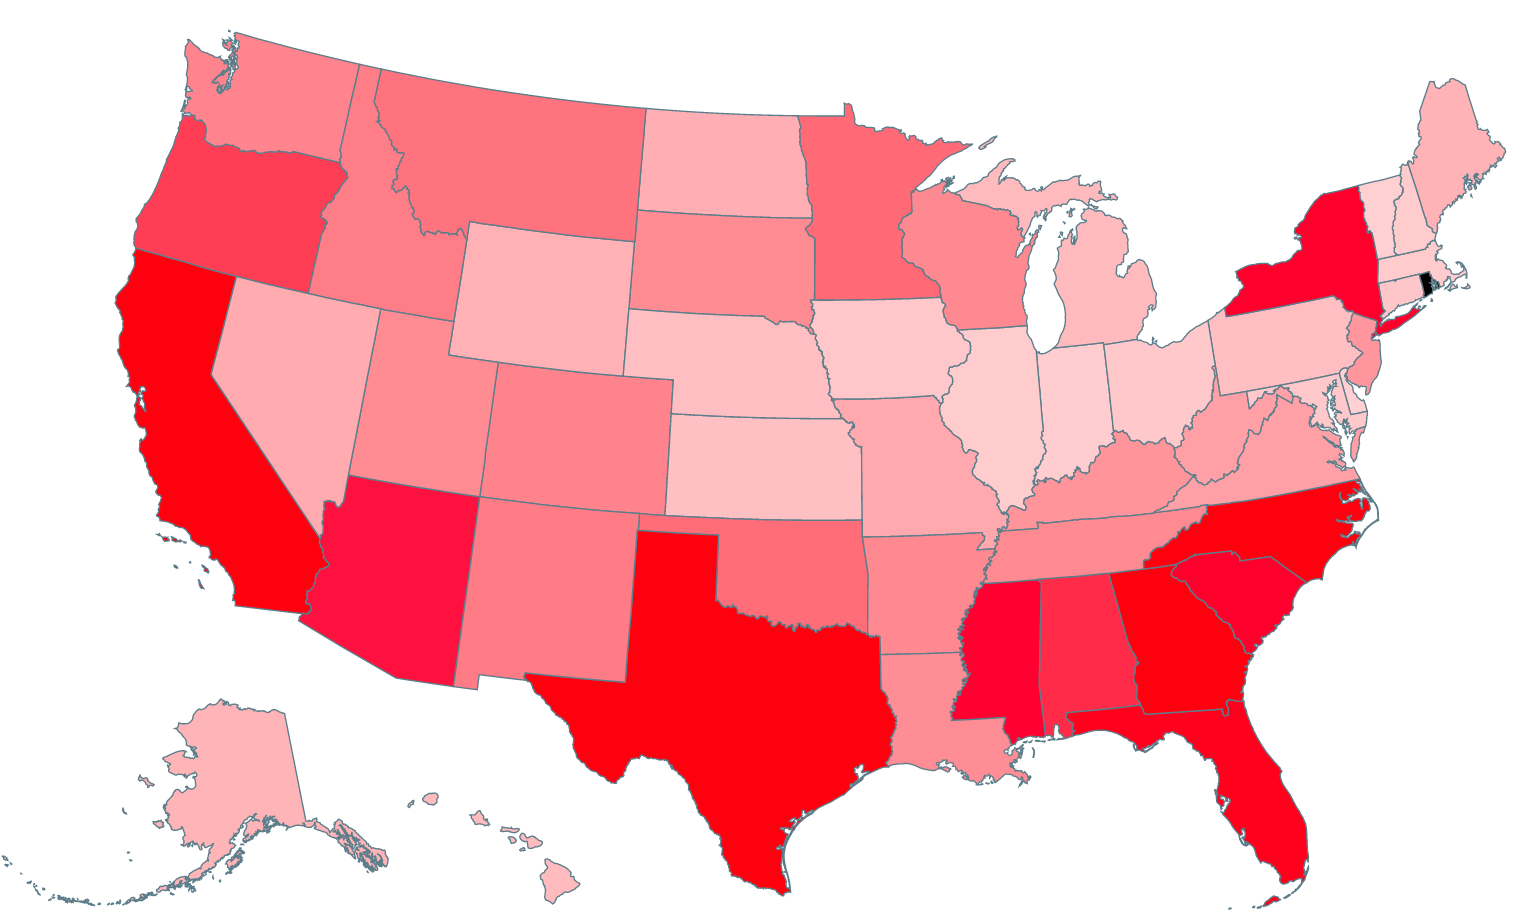
\includegraphics[scale=0.45]{img/choropleth.PNG}
    \caption{Choropleth map gives a representation for the amount of fires in each state. Darker colors represent those states with more fires.}
    \label{fig:choropleth}
\end{figure}

Along with the generation of a choropleth map, the Google Maps API was used to visualize the wildfire clusters in the dataset. Upon requesting access for the Google Maps JavaScript API, Google provided an API key, which was embedded into the web client frontend code. Then, a ReactJS wrapper for interacting with the Google Maps API was used to embed a map object into the page and denote clusters based on markers generated from the latitude and longitude coordinates present in the data. These clusters can be clicked on and zoomed in to find the exact location reported for each fire entry. A high-level overview of the clusters seen in the Google Map object can be seen in Figure \ref{fig:google_maps_clusters}.

\begin{figure}
    \centering
    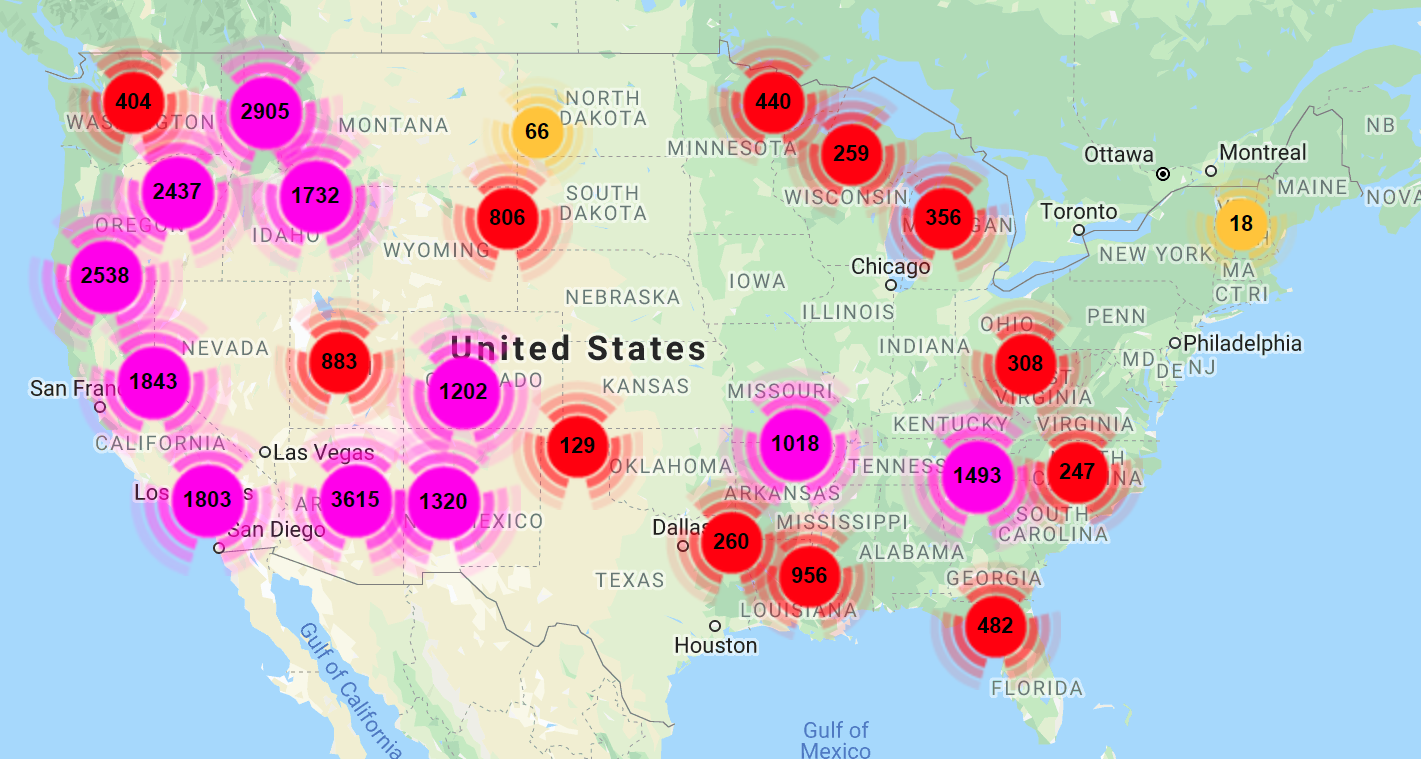
\includegraphics[scale=0.44]{img/google_maps_clusters.PNG}
    \caption{Fire clusters denoted in Google Maps. This visualization is interactive and allows for StreetView and zooming into individual fire locations.}
    \label{fig:google_maps_clusters}
\end{figure}

A donut chart was also generated using the ChartJS library. It represents the frequency of the various causes of fires. This chart can be seen in Figure \ref{fig:donut_chart}. It represents information similar to that in Figure \ref{fig:fire_causes} from the data exploration, but in a more understandable form. \par

\begin{figure}
    \centering
    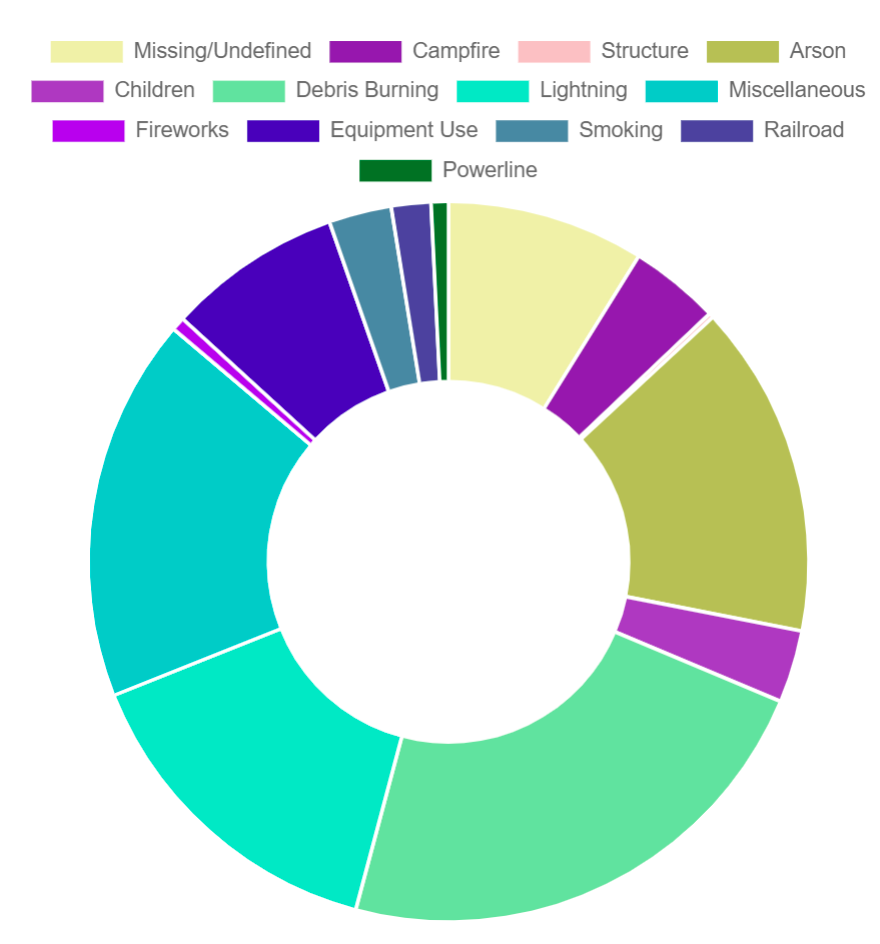
\includegraphics[scale=0.7]{img/donut.PNG}
    \caption{Donut chart represents the frequency of the different causes for fires.}
    \label{fig:donut_chart}
\end{figure}

All of these visualizations are provided properties on render. This means that they can easily be changed based on parameters of interest. A modular design choice such as this allows for visualizations to be dynamically created given any user input. \par

\subsection{Machine Learning}
In terms of Machine learning, the model was trained using a suitable machine learning algorithm so as to predict the causes of wildfire. After the exploratory data analysis, the Naïve Bayes Classifier algorithm was first implemented as it is said to give strong independent assumptions between the features giving a strong motivation to start with this algorithm. The model trained by using this method did not give a good accuracy, which gave a clear indication to move on to some algorithm better tailored for the data. \par

Next, the Decision Trees algorithm was implemented as it uses a tree like model of decisions to give possible chance event outcomes. The target was to predict such chance-event possibilities when this algorithm is implemented on the model. Still, the expected accuracy was not achieved as there was no considerable improvement due to decision trees inability to handle the features that our dataset had. \par

Finally, the Random Forest Classifier Algorithm, as shown in Figure \ref{fig:random_forest}, was employed. It comprises of many decision trees, and hence, provides ease in feature handling. This algorithm uses bagging and feature randomness when building each individual tree to try to create an uncorrected forest of trees whose prediction by committee is more accurate than that of any individual tree. This algorithm gave us a decent accuracy thereby reproducing legible predictions about the probable causes of wildfires. After this algorithm was implemented, to make the model more user-friendly, the user was allowed to provide inputs such as latitude, longitude, month and day of week of their choice so as to let them see the dynamic predictions made by the model in the form of a histogram as depicted in Figure \ref{fig:model_predictions}.

\begin{figure}
    \centering
    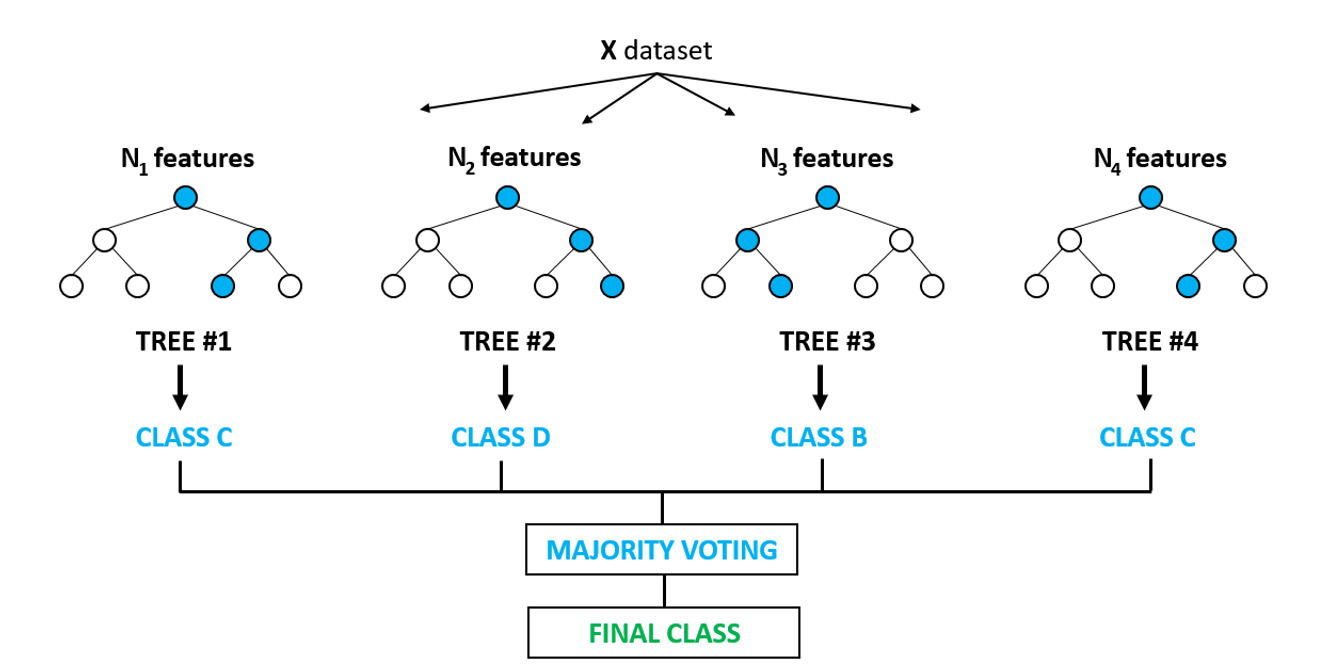
\includegraphics[scale=0.55]{img/random_forest.PNG}
    \caption{Structure of the random forest machine learning model. It includes multiple embedded decision trees for efficient and accurate classification of the feature space.}
    \label{fig:random_forest}
\end{figure}

\subsection{Cloud Deployment}
The cloud deployment of the application poses some interesting issues that need to be overcome. \par

First, it is important to choose a viable cloud service provider from the many prominent companies offering cloud infrastructure. As this project was completed for educational purposes, the deployment needed to be done on the free tier of these commercial services. Both Amazon and Google provide competitive resource quotas in the free tier. Thus, most of the deployment is done with these two companies. \par

Additionally, a few portions of the application are dependent on the Google Maps API. This leads to a security concern regarding the API token allowing access to the platform. Thus, it was important to consider environment variable dependency injection in the Flask application. As this was deployed with Amazon Elastic Beanstalk, it was quite straightforward to manually provide the keys after deployment. Similarly, the connection endpoint and credentials needed to be provided for the MongoDB cluster holding the entire dataset. This was also done as an environment variable injection. \par

Along with security measures, it was important to minimize development time while using the cloud platform so as to avoid incurring extra fees. Thus, a majority of the development was done on local platforms and only the final implementation was pushed into the cloud. While the application was taken down after a live demo, the procedure is documented in the open-source GitHub repository, which can be found in Appendix \ref{appendix:Links}.

\section{System}
\subsection{Software Structure}
The software architecture for this wildfire visualization and prediction web application is given in Figure \ref{fig:software_architecture}.

\begin{figure}
    \centering
    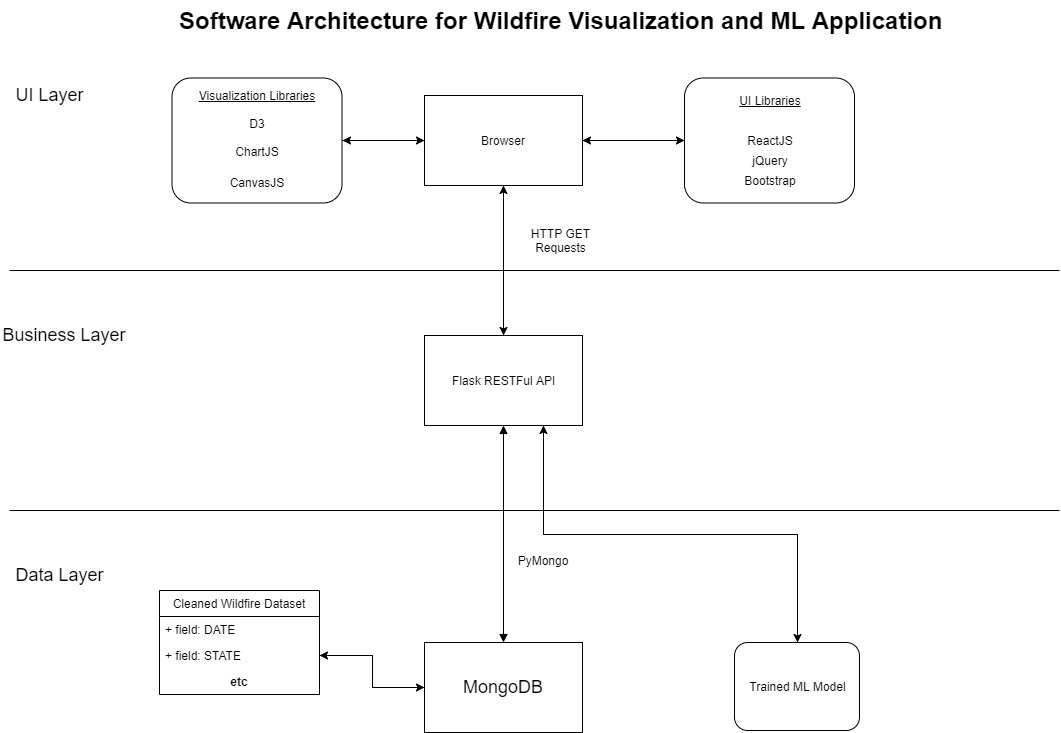
\includegraphics[scale=0.2]{img/software_architecture.jpg}
    \caption{Software architecture for the wildfire prediction and visualization system. The web application has been deployed using cloud services.}
    \label{fig:software_architecture}
\end{figure}

Clearly, there are many moving parts for this system. However, all of the components can be succinctly split into the Data Layer, Business Layer, and Frontend Layer. All of these components are then deployed using cloud services and exposed over the internet. \par

\subsection{Data Layer}
The cleaned dataset is stored in a NoSQL database. For this implementation, MongoDB provided a suitable document-based hierarchical database structure for the data. It was also chosen for its ability to easily manipulate and parse large datasets. \par

MongoDB's PyMongo client library allows Python libraries to easily query the data stored in the database and perform operations on the results. Particularly, the aggregate functionality is used for many of the visualizations. This is an alternative to the MapReduce methods of MongoDB which also allow for high volumes of data to be easily mapped, projected, and aggregated. Both of these methods are quite useful for operations such as counting the number of documents given certain parameters. \par

\subsection{Business Layer}
The main logic of the application is in the form of a RESTful application program interface (API) written with the Flask library in Python. This was chosen to allow any type of HTTP-based client access to the machine learning models. Thus, while the application in this implementation is written for a browser, the platform is not limited solely to web browsers. \par

Flask allows for the definition of multiple routes. The main routes for this system are /api/visualization and /api/prediction. \par

The visualization endpoint supports GET requests with query parameters from the client side. Upon receiving a request for a visualization, the Python application parses the query parameters and communicates with the MongoDB server through the PyMongo library. Then, the results to the request are stored into a JSON format and sent back to the client. \par

The prediction route, on the other hand, provides support for POST requests which include user-defined parameters. These parameters are then run against a trained model and the predictions for causes are returned in the form of a JSON string. \par

This approach allows for easy extensions to the API in the form of new routes. Additionally, all of the database connection is encapsulated into this program. Thus, the client is not required to know how to interact with MongoDB to pull documents out of the database. Additionally, the machine learning models can be easily updated and modified without breaking functionality. Hence, this design scheme follows the separation of concerns ideology. \par

\subsection{Frontend Layer}
The frontend is developed in ReactJS, which is a JavaScript framework for quick web application design. ReactJS was chosen for its modular, component-based approach. This allows for selective document object model (DOM) rendering, which is particularly useful due to the large number of data points necessary for each visualization. \par

Furthermore, ReactJS provides easy integration with the Axios request library. This is used to send GET requests to the RESTful API and pull the data required for whichever visualization is being rendered as well as the results for any predictions made by the machine learning model. All of the data is received in the form of a JSON string and decoded into a JavaScript JSON object for easy data manipulation. \par

The application is built using a single page approach and follows from an administration panel template. The sidebar has two buttons to delineate the the major sections of the application: exploratory visualization and machine learning. The exploratory visualization section of the webpage can be seen in Figure \ref{fig:web_layout_visualization}; similarly, the layout of the machine learning portion can be seen in Figure \ref{fig:web_layout_ml}. \par

\begin{figure}
    \centering
    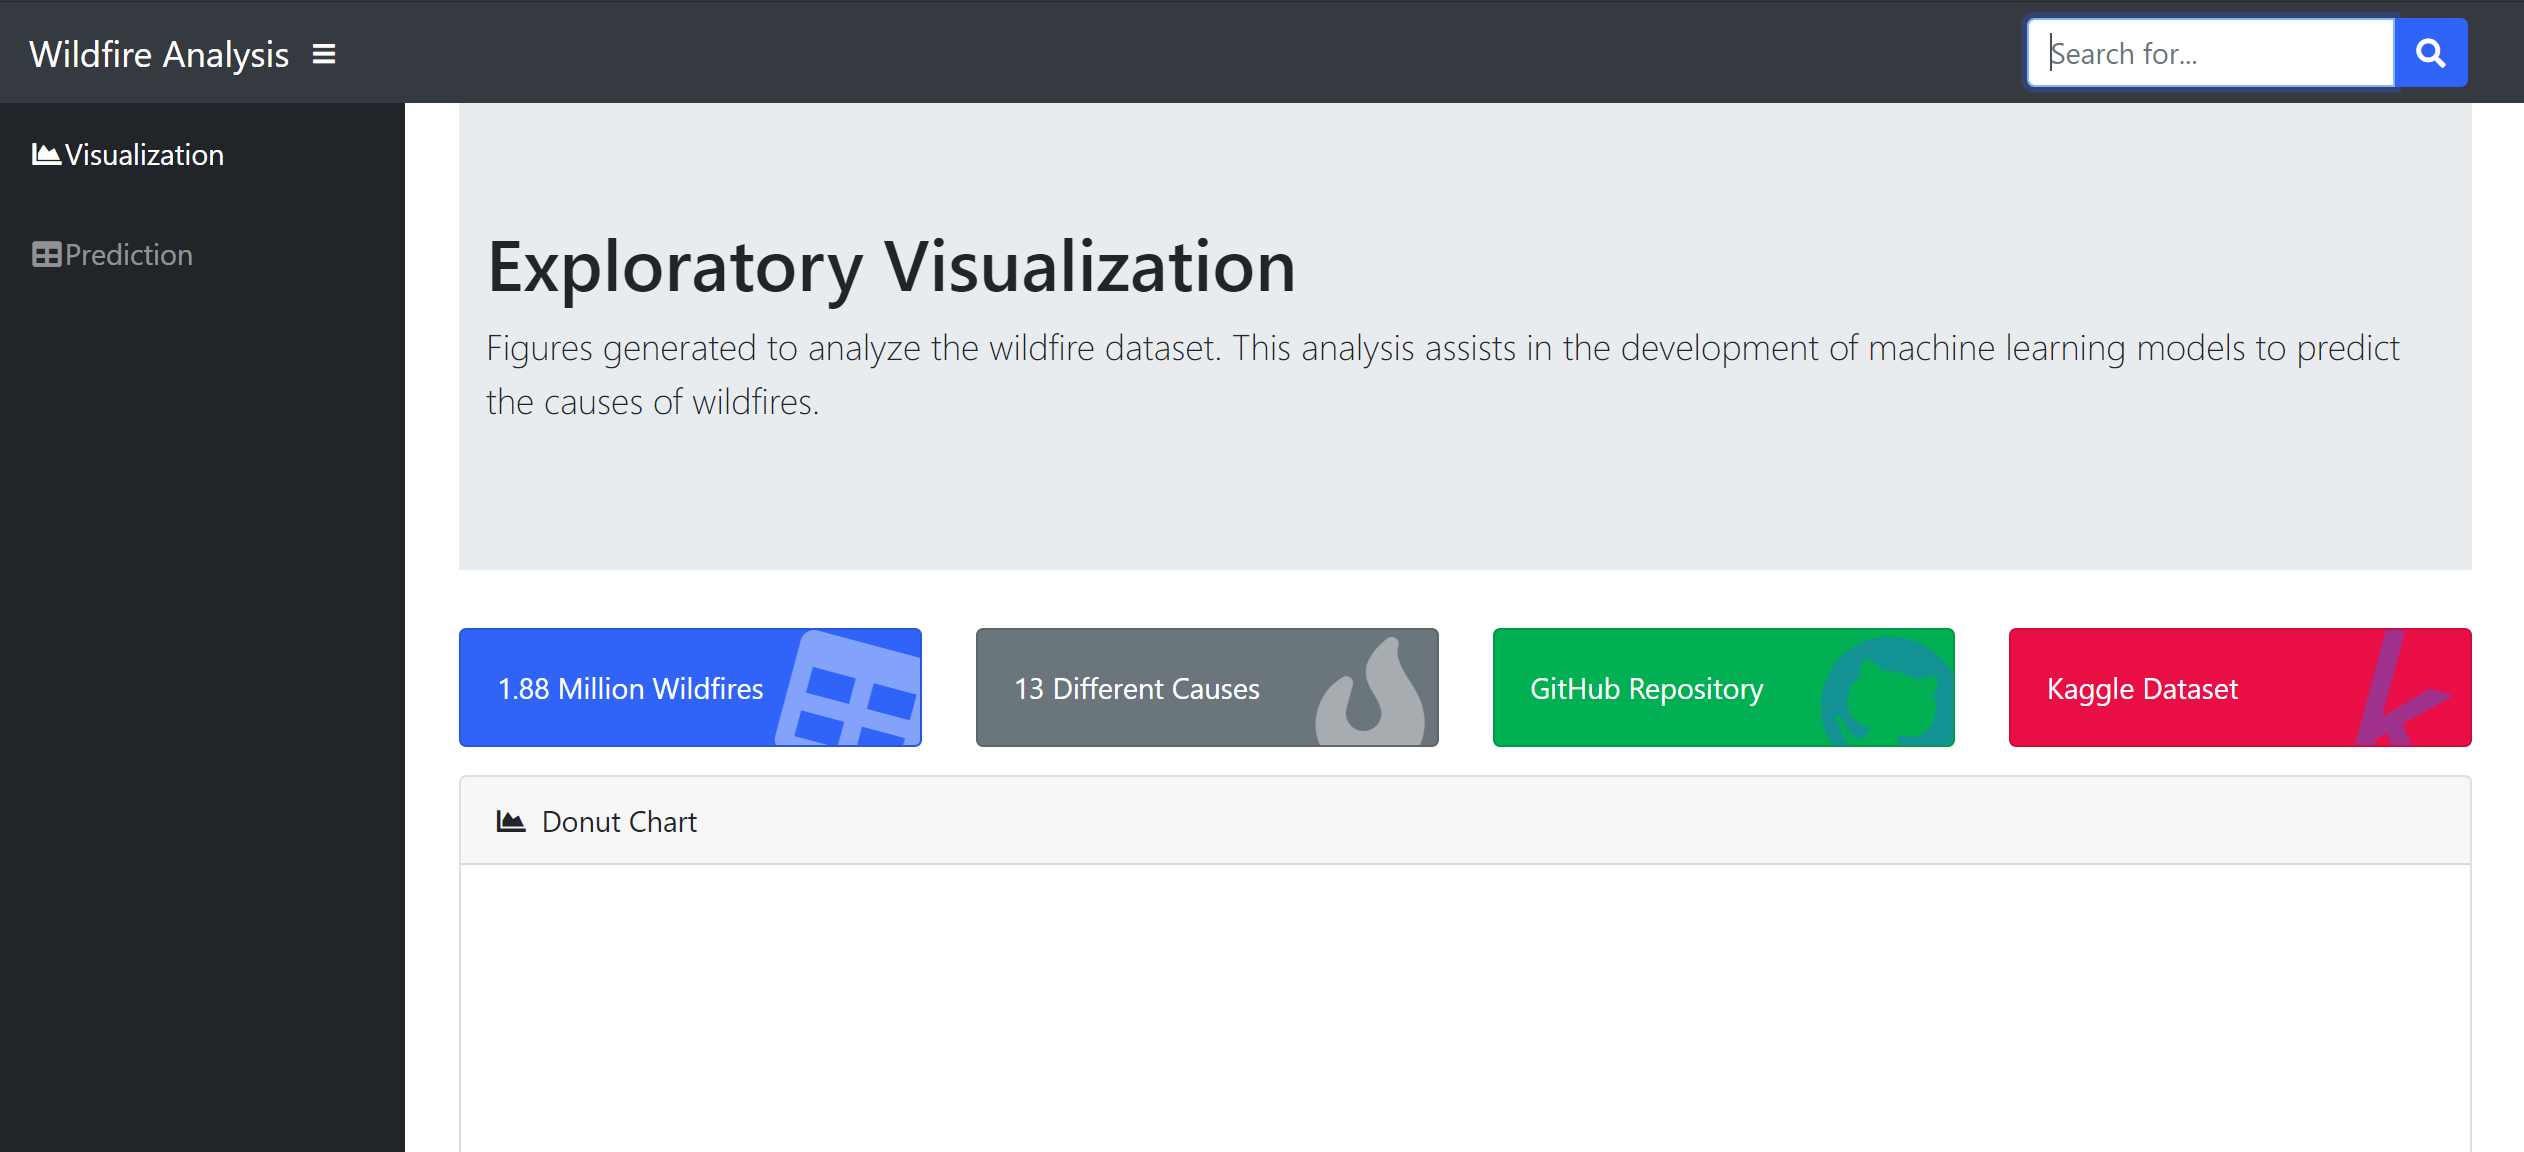
\includegraphics[scale=0.2]{img/web_layout_visualization.PNG}
    \caption{Layout of the exploratory visualization page of the website. The icon cards contain relevant links and the static and dynamic visualizations can be seen lower on the page.}
    \label{fig:web_layout_visualization}
\end{figure}

\begin{figure}
    \centering
    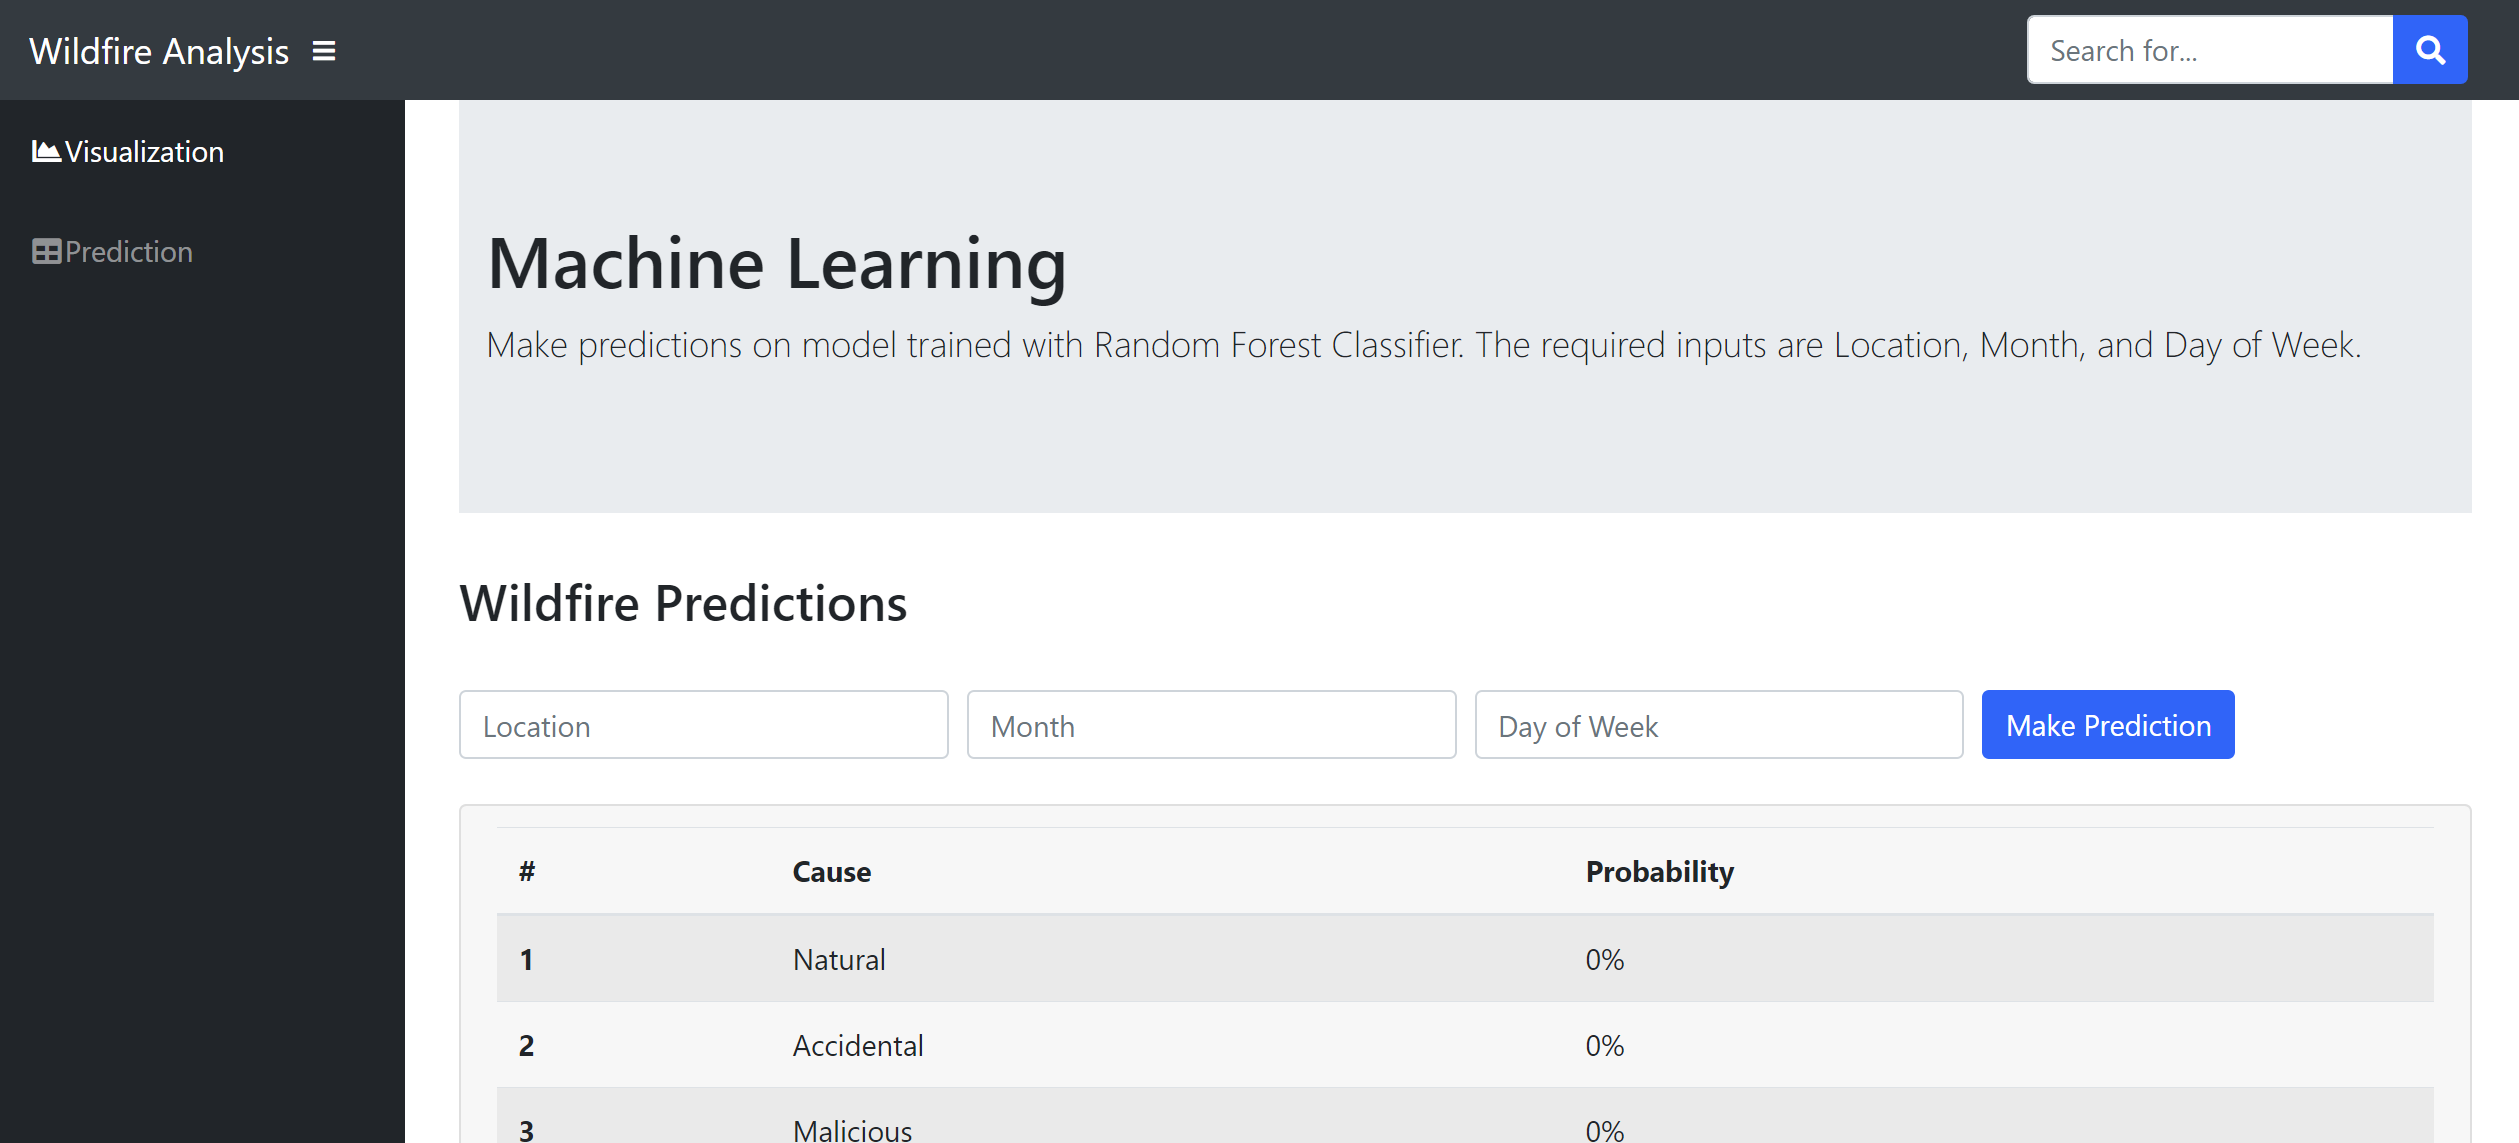
\includegraphics[scale=0.2]{img/web_layout_ml.PNG}
    \caption{Layout for machine learning portion of the website. The inputs allow the user to provide a Location, Month, and Day of Week. The output predictions for wildfire cause are given below in tabular and chart formats.}
    \label{fig:web_layout_ml}
\end{figure}

The visualization section provides a series of fixed visualizations of the aggregate data. This is followed by a user input form with a selection of dynamic visualizations that are generated based on the user's choices. \par

The machine learning part of the application provides distinct input sections so users can perform operations on the model trained to predict wildfire causes. Once a user inputs the parameters of a wildfire and submits the form, the application applies the parameters to the selected model and returns the likelihoods for the aforementioned fire cause categories. \par

\subsection{Cloud Service Structure}
Many considerations were made for the cloud deployment infrastructure. As of this writing, the most commonly used cloud service providers are Amazon Web Services (AWS), Google Cloud, and Microsoft Azure. \par

This application's RESTful API was deployed using the Elastic Beanstalk service from AWS in a Flask environment running on Python 3. This is essentially a platform as a service (PaaS) system from Amazon which provides managed compute engines and dependency injection. It was chosen for the ability to deploy quickly without any user-defined hardware management. \par

The database was instantiated in a MongoDB Atlas cluster serviced by Google Cloud. Since this is a big data application, the free tier, which provides 500 megabytes of storage, is not sufficient. Thus, the smallest paid database cluster was used for a proof-of-concept implementation. Larger computation infrastructure would be needed for faster look ups and to support multiple clients. \par

The static files required for the frontend of the application were served in an Amazon Simple Storage Service (S3) bucket with public web hosting. This allows for GitHub pipeline integration which is useful to quickly push any updates to the design and make them live without any delays. A screenshot of the model and website files uploaded into the S3 bucket can be seen in Figure \ref{fig:s3_upload} \par

\begin{figure}
    \centering
    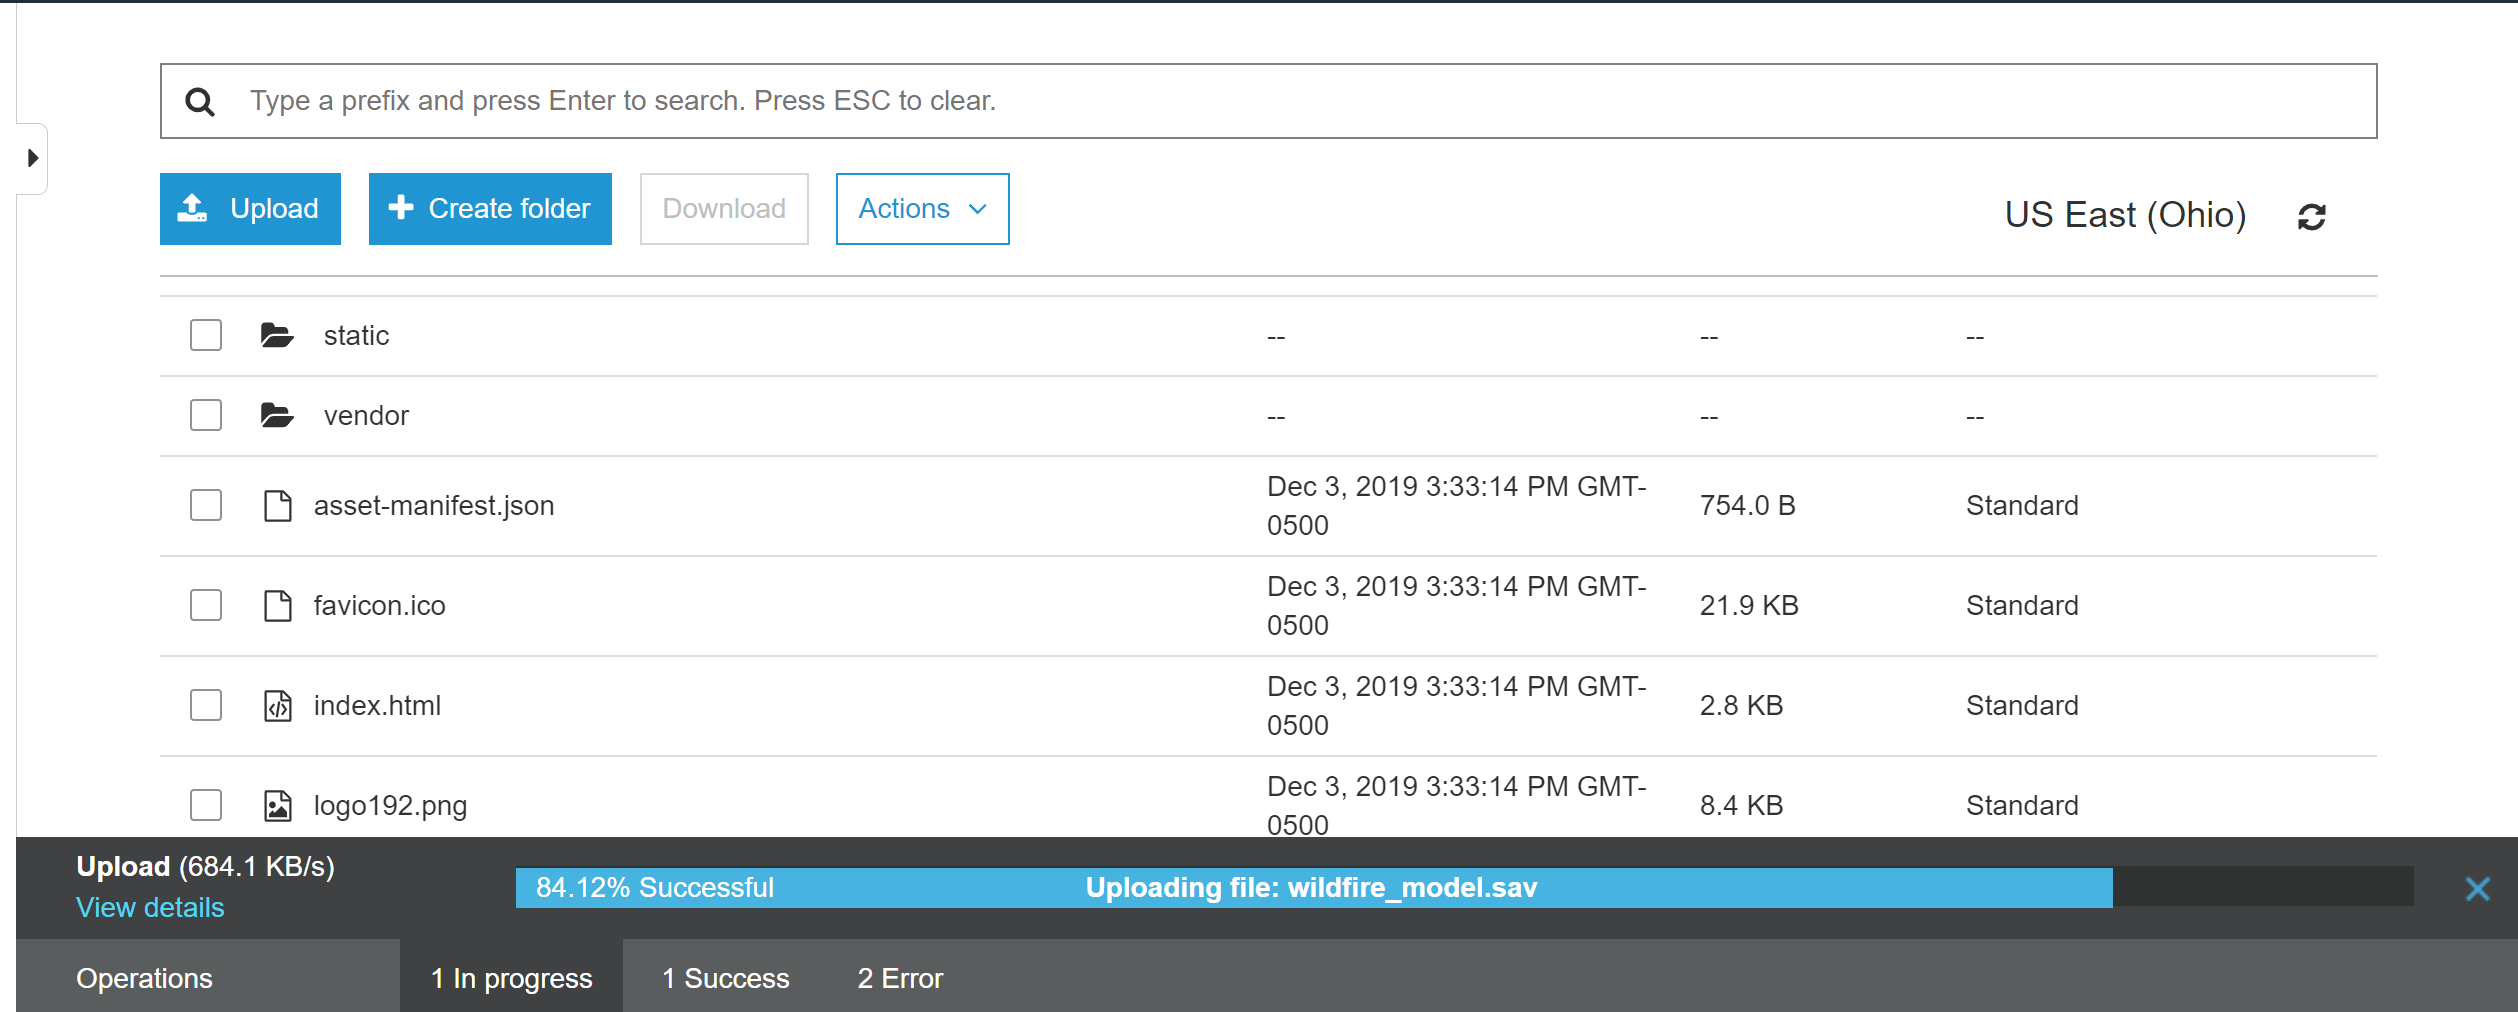
\includegraphics[scale=0.26]{img/s3_upload.PNG}
    \caption{Screenshot of frontend files and machine learning model in Amazon S3 bucket.}
    \label{fig:s3_upload}
\end{figure}

In a large scale deployment, all of these systems would be put behind a load balancing service, API gateway, and caching distribution. This would allow for one endpoint that all clients can connect to. Additionally, the caching distribution would allow for static content to be cached for faster access and the API gateway would allow for authentication if the system were to be commercialized. \par

\section{Conclusion}
Wildfires have tremendous impact in the United States. Every year, fires cause great loss of life and property. Government agencies have publicly released data providing information about these wildfires, including, but not limited to, their location, date of discovery, cause. \par

This project aims to use a dataset of 24 years of wildfire data to create visualizations to analyze and understand the scope and relationships between various features of the data. Using this understanding, machine learning models are created to predict the causes of wildfires given user input. \par

The data has been manipulated and cleaned to allow for reasonable analysis of the wildfire information. After this, rigorous exploratory analysis has been done to determine correlations and associations between the features present in each wildfire entry. This information was used to influence the creation of accurate machine learning models that allow for wildfire cause prediction given user inputs.

A web application has been created to concisely present the visualizations and machine learning models. The web page allows for users to dynamically generate visualizations for parameters of interest and make cause predictions for possible fires throughout the United States. \par

This project also has great scope for extension. Different models can be created from the data to predict likelihood of fires at certain times of month. Additionally, limitless interesting visualizations can be generated to represent the data in an understandable format. Aside from wildfires, this web application creation and deployment approach can be implemented with other datasets to reveal meaningful results. \par

\section*{Acknowledgment}
The authors gratefully acknowledge the contributions of Professor Ching-Yung Lin of the Electrical Engineering department at Columbia University and TAs Frank Ou Yang, Tingyu Li, Yunan Lu, and Juncai Liu for their insightful input and analysis leading to the creation of this work. \par
Additionally, without Rachael Tatman's compilation of the government wildfire data from Karen C. Short, none of this work would have been possible. \par

%\begin{thebibliography}{00}
%%%% Adding the bibliography from external file
\nocite{*}
\bibliographystyle{IEEEtran} % We choose the "IEEEtran" reference style
\bibliography{references} % Entries are in the "references.bib" file
%\end{thebibliography}

 \appendices

\section{Links}
\label{appendix:Links}
The source code created in the development of this project can be found on GitHub at \url{https://github.com/SidBambah/Wildfire-Prediction-Visualization-ML}. \par

The YouTube video created to demo the software and give an overview can be found at \url{https://youtu.be/aAZ1EnyyqEk}.\par
  
\vspace{12pt}

\end{document}